\section{Primer on programmable switch architectures}
\label{s:architecture}

\begin{figure*}[t]
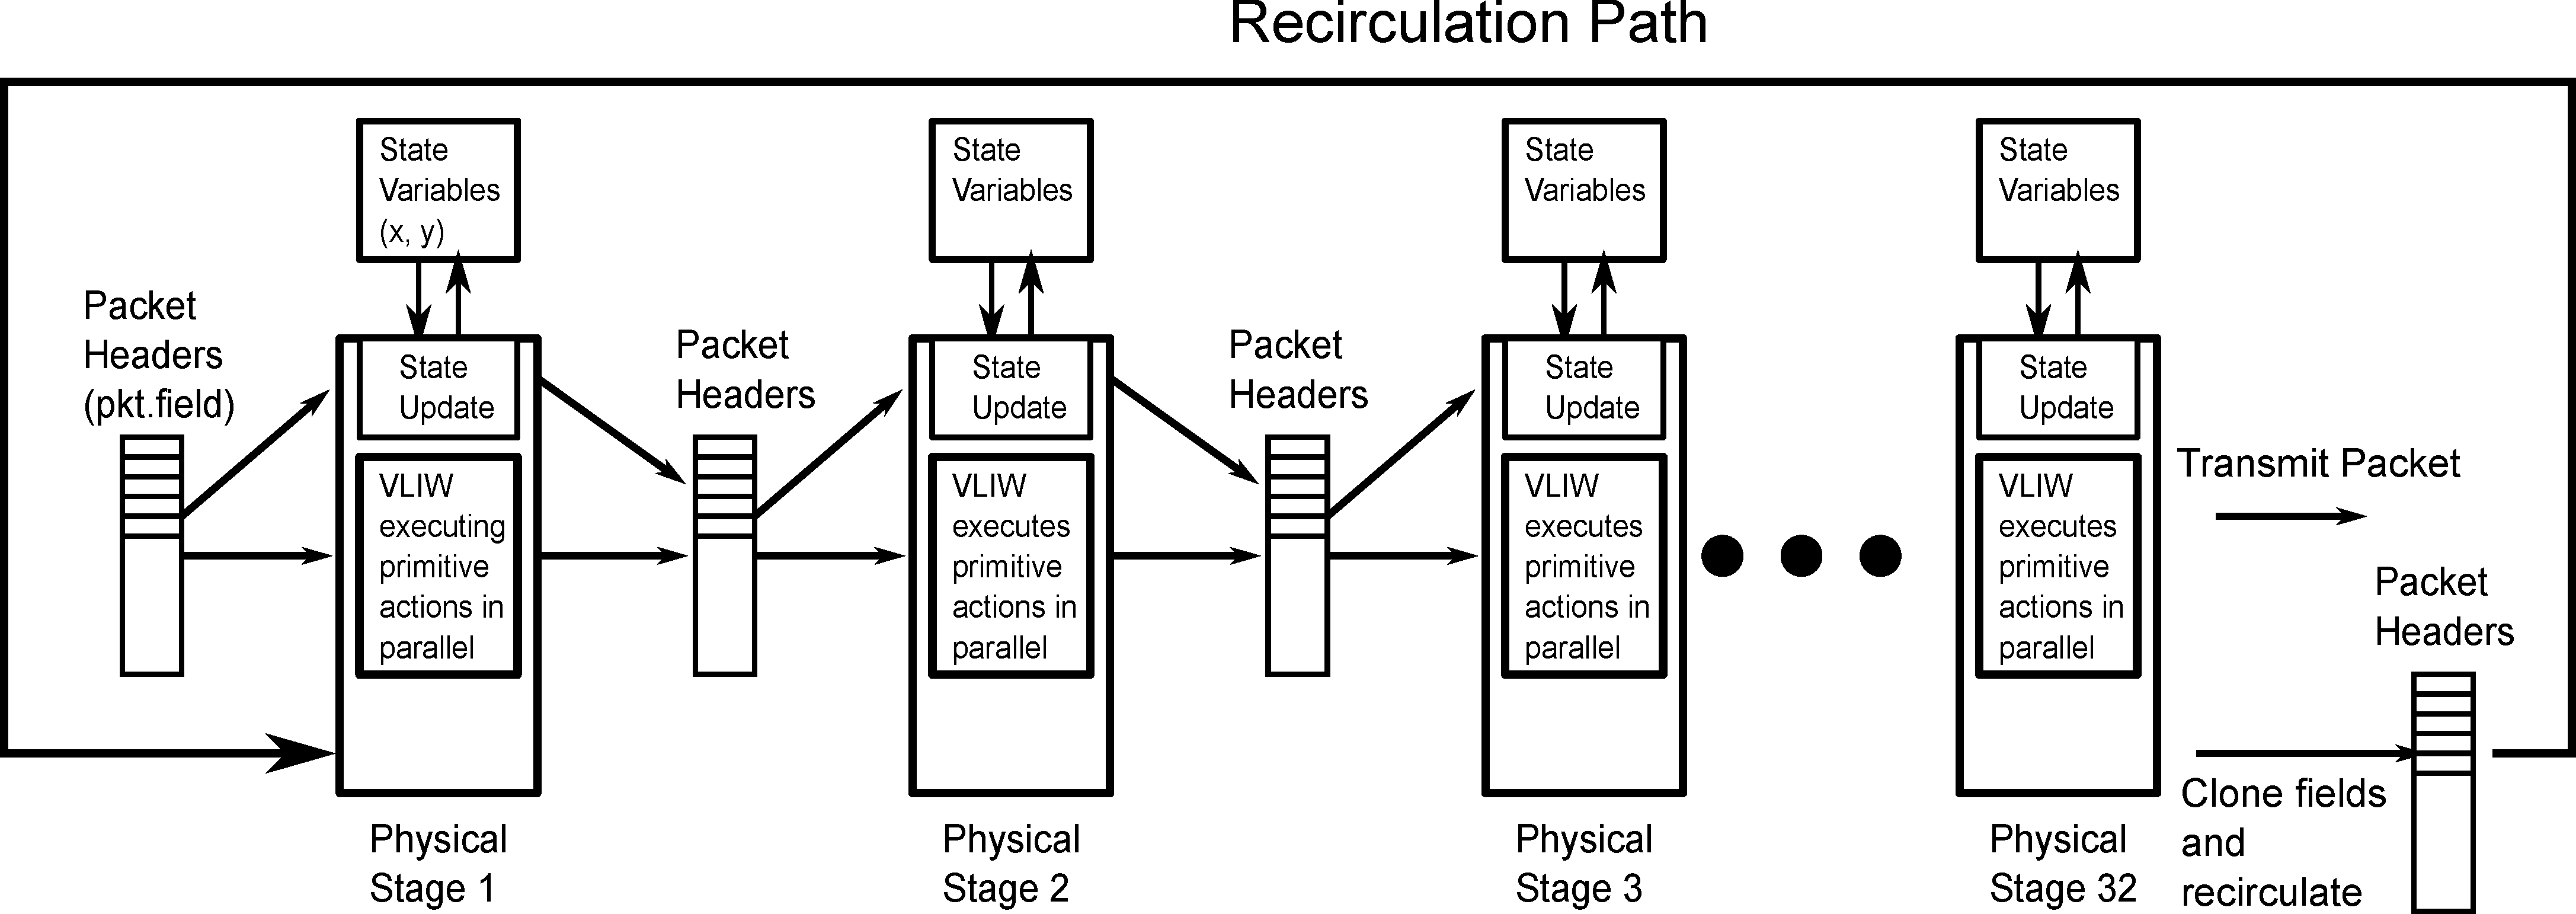
\includegraphics[width=\textwidth]{p4_switch_model.pdf}
\caption{The protocol-independent switch architecture implemented in the
abstract machine banzai.}
\label{fig:architecture}
\end{figure*}

This section provides a brief primer on the architecture of a programmable
switch to provide sufficient context for the rest of the paper. For
concreteness, we describe an idealization of a protocol-independent switch
architecture~\cite{pisa} that we implement as an abstract machine, banzai, for
this paper.

banzai captures features of programmable switches such as the Reconfigurable
Match-Action Table (RMT) architecture~\cite{rmt}, Intel's
FlexPipe~\cite{flexpipe} and Cavium's Xpliant~\cite{xpliant}. Because banzai is
an abstract machine, we model mechanisms that are critical to mapping
data-plane algorithms and abstract out details such as match-action tables, and
packet parsing. We later show(\S\ref{s:section}) how domino can be integrated
into a switch compilation pipeline that targets switches with match-action tables
by using P4 as a backend.

banzai assumes that packets entering a programmable switch have been  parsed by
a programmable parser that turns packets into a set of header fields. The set
of packet headers is processed by an ingress pipeline consisting of
match-action tables arranged in stages. The packet then enters the switch
scheduler, and once it has exited the scheduler, it is processed by a similar
egress pipeline. banzai models a generic packet-processing pipeline, with the
only distinction between ingress and egress being the set of packet headers
available at the entrace of each pipeline.

Packet processing itself happens within the stages contained inside these
pipelines. Each stage contains a vector of atoms: a body of code that process
and modify a packet and complete execution before the next packet arrives at
the stage.  An atom may also contain hidden state that can influence the atom's
behavior from one packet to the next. An example of a counter that could be
written as an atom as follows (we use the notation to p(``x'') to represent access
to field ``x'' within a packet or state variable ``x''.
\begin{verbatim}
void counter(Packet & p, State & s) {
  p("tmp")     = s("counter");
  p("tmp2")    = p("tmp") + 1;
  p("count")   = p("tmp2");
  s("counter") = p("tmp2");
}
\end{verbatim}

banzai is a shared-nothing architecture: state variables are local to a
particular atom and can only be shared with atoms in subsequent stages by using
packet fields.  This restriction reflects the capabilities of most switches
today: building memories that can be simultaneously accessed from multiple
switch stages is technically challenging.  To let a stage communicate state
information to a predecessor stage upstream, banzai allows packets to be cloned
and recirculated back into a pipeline, modeling the loopback interfaces found
on most switches today.

This way, a state variable $x$ can be read in an atom $A$ in stage 1, written
downstream in stage 2, and then a cloned packet to stage 1 could update the
state variable $x$ in $A$.  However, recirculation has a cost: recirculated
packets consume pipeline capacity by taking away capacity from new data
packets. Further, recirculation latency can be large: several hundred packets
might pass through the pipeline before the recirculated packet updates state in
$A$.

{\textbf Restrictions on atom bodies}
For any high-performance switch that is to operate at an aggregate forwarding
capacity exceeding a Terabit / sec, we need to restrict the complexity of each
statement within the atom and the number of statements within each atom.

To restrict the complexity of each statement, we assume each statement can
carry out simple stateless arithmetic operations (add/sub/shift) on packet
fields. Further, many atoms can execute in parallel using a Very Large
Instruction Word that carries out operations on distinct header fields in
parallel.

To restrict the length of each atom, we note that each atom needs to be
implemented in hardware using an underlying combinational circuit. We describe
(\S\ref{s:mapper}) a mapping procedure that converts sequential code blocks to
configurations of combinational circuits, rejecting atoms that cannot be mapped
to the combinational circuit. We next describe the combinational circuit that
we use for the rest of the paper.

{\textbf The combinational circuit implementing atoms}
At a high level, the combinational circuit represents the limit on useful
packet and state modifications between two packets arriving back-to-back on a
high-performance switch pipeline. These switch pipelines operate at close to 1
Ghz ~\cite{rmt}, implying that the effective budget for packet and state
modifications is about 1 ns.

Keeping this time budget in mind, we assume that the circuit can read, modify,
and write at most two addresses in stateful memory, where the modification to
each address might depend on the previous value in the other address and from
values in at most two packet fields. To restrict the complexity of
modifications, we restrict each stateful modification to a predicated
instruction that can conditionally modify each address based on the value of
the same or another address.

For concreteness, we describe the combinational circuit as an imperative
program below. We use the following notation:
\begin{enumerate}
\item \texttt{state\_hi} and \texttt{state\_lo} refer to two stateful addresses.
\item \texttt{packet\_hi} and \texttt{packet\_lo} refer to two packet fields.
\item \texttt{\{a,b,c\}} denotes the fact that either a, b, or c could be used
in a particular location.
\item \texttt{math} denotes a pure mathematical function approximated as a lookup
  table.
\end{enumerate}

\begin{tiny}
\begin{verbatim}
// Predicates for updates to state
bool condition_a = {+,-} {state_hi, state_lo} {+,-} {packet_hi, packet_lo} + constant {<=, <, ==, !=, >, >=} 0;
bool condition_b = {+,-} {state_hi, state_lo} {+,-} {packet_hi, packet_lo} + constant {<=, <, ==, !=, >, >=} 0;

// Compute one-hot mask from predicates
bool[4] one_hot_mask = compute_one_hot_mask_from condition_a_and_condition_b(condition_a, condition_b);
bool state_hi_alu1_ran = false;

// Execute state_hi's ALUs based on the predicate
int state_hi_alu1_result = 0;
if (state_hi_alu1_mask & one_hot_mask) {
  state_hi_alu1_result = {state_hi, state_lo, constant, math{state_hi, state_lo}} {+, -, min, max} {packet_hi, packet_lo, constant};
  state_hi_alu1_ran = true;
}

int state_hi_alu2_result = 0;
if (state_hi_alu2_mask & one_hot_mask) {
  state_hi_alu1_result = {state_hi, state_lo, constant, math{state_hi, state_lo}} {+, -, min, max} {packet_hi, packet_lo, constant};
  state_hi_alu1_ran = true;
}

// Combine results from both ALUs
if (!state_hi_alu1_ran && !state_hi_alu2_ran) {
  state_hi_alu_result = state_hi;
} else {
  state_hi_alu_result = state_hi_alu1_result | state_hi_alu2_result;
}

// Execute state_lo's ALUs based on the predicate
int state_lo_alu1_result;
if (state_lo_alu1_mask & one_hot_mask) {
  state_lo_alu1_result = {state_hi, state_lo, constant, math{state_hi, state_lo}} {+, -, min, max} {packet_hi, packet_lo, constant};
  state_lo_alu1_ran = true;
}

int state_lo_alu2_result;
if (state_lo_alu2_mask & one_hot_mask) {
  state_lo_alu1_result = {state_hi, state_lo, constant, math{state_hi, state_lo}} {+, -, min, max} {packet_hi, packet_lo, constant};
  state_lo_alu1_ran = true;
}

// Combine results from both ALUs
if (!state_lo_alu1_ran && !state_lo_alu2_ran) {
  state_lo_alu_result = state_lo;
} else {
  state_lo_alu_result = state_lo_alu1_result | state_lo_alu2_result;
}


// Write back results to state_lo and state_hi
state_hi = state_hi_alu_result;
state_lo = state_lo_alu_result;

\end{verbatim}
\end{tiny}
